\section{Frequency Calibration of Local Oscillators}~\label{sec:calib}

The Q-Pix calibration requirements are described in detail in Section~\ref{sec:qpix_circuit}.
The important parameters which must be calibrated for each pixel are the charge per reset and the frequency of the local oscillator.
An aim of this work is to demonstrate an additional frequency calibration method using the minimal required connections between each digital node.

Any method of a frequency calibration must synchronize time measurements between all digital nodes within a tile and the aggregator.
There are several possibile methods to achieve this, but ultimately the data that are recorded must be some time at the aggregator, $T_{a}$, and the time at any specific node, $T_{j}$.

%% distribute clock for calibration of time
A direct method is one where the aggregator distributes its own clock to all nodes in the tile.
This scenario removes the need for a calculation of the frequency of each node altogether since the clock of each node is already known from the aggregator.
This is the simplest case for timing calibration: remove all free running oscillators.

% cross-talk
A distributed clock network indeed removes ambiguity of the remote oscillator frequencies, but at the cost of hardware complexity.
Whether or not this design choice is preferred is entirely detector dependent, but likely increases in difficulty with the scale of the TPC.

We comment, however, that we ignore this scenario because it may altogether be unnecessary depending on future ASIC performance.
In the event that frequency calibrations of sufficient precision ($\bar{f} \approx 1 ppm$) are possible occur on free-running local oscillators future detectors would need only to acquire these ASICs and place them with minimal cost in terms of both time and money.

%% distribute trigger for calibration of time
Another simple scenario is one where the aggregator itself connects directly to all nodes within a tile via a single connection which can be used as a reference trigger.
This means that some trigger from the aggregator would issue directly into each node at the same time: $T_{a} = T_{n}$.
To calcuate the frequency in this manner, the controller would issue two triggers from the aggregator with a known time separation, $T_{o} = T_{a2} - T_{a1}$.
The remote nodes would each record and send their timestamps back to the aggregator, where the time difference would be calculated as:

\begin{equation}
  T_{o} = T_{a2} - T_{a1} = T_{n2} - T_{n1}
\end{equation}

this is rewritten in terms of frequency as follows:
\begin{equation}
  f_{n} = \frac{T_{n2} - T_{n1}}{T_{o}}
\end{equation}

This calibration method, though extremely simple, introduces an additional connection to each ASIC between itself and the aggregator.
For a large scale system such as Q-Pix a single connection per ASIC introduces $\approx 60\times 10^{3}$ hardware points of failure per APA.

Both of these scenarios are valid implementations of a Q-Pix readout system.
In both of these scenarios, however, there is added complexity into the hardware design of the system in the form of additional routing where each route which represents a possible point of failure.

In a world of perfect hardware and costless routing in terms of both time and money these routing schemes would clearly be sufficient.
However, no hardware is perfect.
Therefore we introduce and discuss a calibration technique which relies on no additional routing and could be optionally implemented even in the above schemes in the event of a failure.
Therefore, even if not the primary implemented calibration technqiue, since this calibration introduces no superfluous routing it could still be used regardless of the actual future hardware implementation.

%% distribute packet for calibration of time
\subsection{A Minimal Connection Calibration Procedure}~\label{sec:min_calib}

As stated in the previous section, any frequency calibration records a reference time at the aggregator ($T_{a}$) and an event time ($T_{n}$) at a ASIC within a tile.
The time calibration procedure presented here requires only the minimal routing required in any Q-Pix readout system, where we assume time-dependent free-running local oscillators at each ASIC within the tile.

%% issue 1
The calibration procedure begins at a time ($T_{0}$) where the aggregator sends a calibration packet.

%% recv1
Next, the packet propagates through the tile to some remote ASIC, $N_{j}$.
This ASIC receives the packet later at some time $T_{n1}$:

\begin{equation}
  T_{n1} = T_{o} + T_{f1}
\end{equation}

Where $T_{f1}$ is the propogation time of the packet from the aggregator to the $N_{j}$ ASIC.

%% meas1
This remote ASIC then sends the packet with its time ($T_{n1}$) back to the aggregator.

%% wait
The aggregator will wait some calibration time ($T_{cal}$) before issuing another calibration packet.
This wait period $(\mathcal{O}(10^{0-2})$) can be long compared to the full transaction time to the $N_{j}$ ASIC $(\mathcal{O}(j*10^{-5})$).

%% issue 1
After the wait period, the aggregator will issue a second calibration packet to be sent to a remote ASIC at time:
\begin{equation}
  T_{1} = T_{cal} + T_{0}
\end{equation}

%% recv2 and meas2
Similarly to the first packet this packet will propagate to $N_{j}$ with some new time $T_{f2}$ where $N_{j}$ will record time $T_{n2}$:
\begin{equation}
  T_{n2} = T_{1} + T_{f2}
\end{equation}

Now, we define $\Delta T_{j}$ as the difference in the two time measurements from the two packets sent from the aggregator.
The time difference is related to the number of clocks that occured between the two different measured values of the clock, $T_{n1}$ and $T_{n2}$.

\begin{equation}
  \Delta T_{j} = T_{n2} - T_{n1}
\end{equation}

We use the known relationships for $T_{n2}$ and $T_{n1}$ to obtain:
\begin{equation}
  \Delta T_{j} = (T_{1} + T_{f2}) - (T_{o} + T_{f1}) = (T_{1} - T_{0}) + (T_{f2} - T_{f1}) = T_{cal} + \Delta T_{f}
\end{equation}

Where we defined $\Delta T_{f}$ as the difference in forward propagation times from the packets sent from the aggregator at $T_{1}$ and $T_{0}$.

We arrive at the result which compares the measured time at the aggregator $T_{cal}$ and the time measured at each ASIC, $\Delta T_{j}$:
\begin{equation}
  \Delta T_{j} = T_{cal} + \Delta T_{f}
\end{equation}

A perfect reconstruction of the nodal frequency would follow if $\Delta T_{f} = 0$.
But it is sufficient to note that the wait period happens on the order of seconds, whereas $\Delta T_{f}$ is on the order of $\mu s$ or at least a six order of magnitude difference.
We then use $\Delta T_{f} \ll T_{cal}$ to obtain:
\begin{equation}
  \Delta T_{j} \approx T_{cal}
\end{equation}

We convert time into frequency with the difference of the timestamps measured and a known aggregator frequency ($f_{a}$):
\begin{equation}
   \frac{\Delta N_{j}}{f_{j}} = \frac{\Delta N_{a}}{f_{a}}
\end{equation}

or,
\begin{equation}
   \boxed{f_{j} \simeq \frac{\Delta N_{j}}{\Delta N_{a}}f_{a}}
\end{equation}

Where $\Delta N_{j}$ and $\Delta N_{a}$ are the differences in the timestamps of the 32-bit clocks at the remote node and aggregator, respectively.


\subsubsection{Packet Transaction Time}

 We next examine the approximation that $\Delta T_{f} \ll T_{cal}$ and consider its contribution to the error in the reconstruction of $T_{j}$.
This analysis also provides a constraint on the duration of $T_{cal}$ to ensure an accurate measurement of each $T_{j}$ in a tile.
We begin by discussing how long it takes for a packet to traverse a tile.

The time it takes for each packet to be received by the next node is given in Equation~\ref{eq:t_packet}.
The value, $N_{bit}$, is the number of clock cycles used for the packet and is protocol-dependent.
Since the protocol must be deterministic for each packet, $N_{bits}$ must be the same for each transaction on the path from the base-node to the remote node.

As an example, the time it takes for a packet to go from the base-node, $N_{1}$, to a remote node, $N_{3}$, via the path $1\rightarrow 2 \rightarrow 3$ is determined by:
%% packet transaction time
\begin{equation}
  T_{1\rightarrow 3} = T_{1\rightarrow 2} + T_{2\rightarrow 3} \approx \frac{N_{bits}}{f_{1}} + \frac{N_{bits}}{f_{2}} = N_{bits}(\frac{1}{f_{1}} + \frac{1}{f_{2}})
\end{equation}~\label{eq:t_packetTransfer}

Where, $f_{i}$, is the frequency of the clock at sending node. The approximation is within a single clock cycle of the receiving digital node ($\approx 33~\unit{ns}$).

Therefore the time it takes for a packet for go from the base-node to any remote node is proportional to $N_{bits}$ multiplied by the sum of the edges in the full adjacency matrix given by Equation~\ref{eq:adjacency_comp}.

We generalize Equation~\ref{eq:t_packetTransfer} to represent the time it takes a packet to go from the aggregator ($i = 0$) to any remote node, $N_{j}$:
\begin{equation}
  T_{f} = T_{0\rightarrow j} = N_{bits}\sum_{i=0}^{i=j-1}\frac{1}{f_{i}}
\end{equation}

We require that every calibration packet on the protocol uses the same number of clocks ($N_{bits}$ is constant) and follows the same path. $\Delta T_{f}$ becomes:
\begin{equation}
  \Delta T_{f} = N_{bits}\sum_{i=0}^{i=j-1}\frac{1}{\Delta f_{i}} = N_{bits} \sum_{i=0}^{i=j-1}\Delta T_{i}
\end{equation}

We recognize $\Delta T_{i}$ as the nominal time-dependent clock drift of the each local oscillator in the path between the base-node to the remote-node.
We can provide an order of magnitude estimate for $\Delta T_{f}$ if we assume a (very poor) $\approx 1\%$ drift in each of the remote clocks within the tile during a period of $T_{cal} \approx 1~\unit{s}$.
In this approximation we also assume that the mean of the periods of the nodes are the designed value ($\approx 33~\unit{ns}$) for which a 1\% error gives $\sigma_{T_{f}} \approx 3~\unit{ps}$.
If we assume that all of the clocks (for whatever reason) drift have error which drifts int he same direction (the sum doesn't cancel) then for 100 transactions with 1000 clocks per transaction, we obtain for $\Delta T_{f}$:
\begin{equation}
  \Delta T_{f} \approx 1000 * 100 * 3\times 10^{-12} \approx 30~\unit{ns} \ll 1~\unit{s} \simeq T_{cal}
\end{equation}

\section{The Digital Prototype Design}~\label{sec:qdb_prototype}
%% QDB Hardware Discussion

This section marks the second part of this chapter.
We describe the design of a modular digital back-end prototype board
The results presented here construct a tile 4$\times$4 array of Lattice ice40UP5k FPGAs.
Each FPGA is programmed with the logic described in the previous sections.

These nodes are used to test the cotrol logic, communication stability, buffer requirements, and calibration procedure which will be tested in the future Q-Pix digital prototype ASIC.
The most important quantity to be calibrated for the digital nodes is the frequency of the local oscillator.
The Q-Pix reconstruction for both time and z position are dependent on this parameter, see Chapter~\ref{chap:qpix}.

Future implementations of the digital back-end for Q-Pix may, of course, use different oscillators.
However, these results are still beneficial as a proof of concept for the frequency calibration, as well as tests to the packet loss susceptibility.
Packet loss is a function of relative frequency drift between neighbor nodes.

\begin{figure}
\centering
\begin{subfigure}{.5\textwidth}
  \centering
  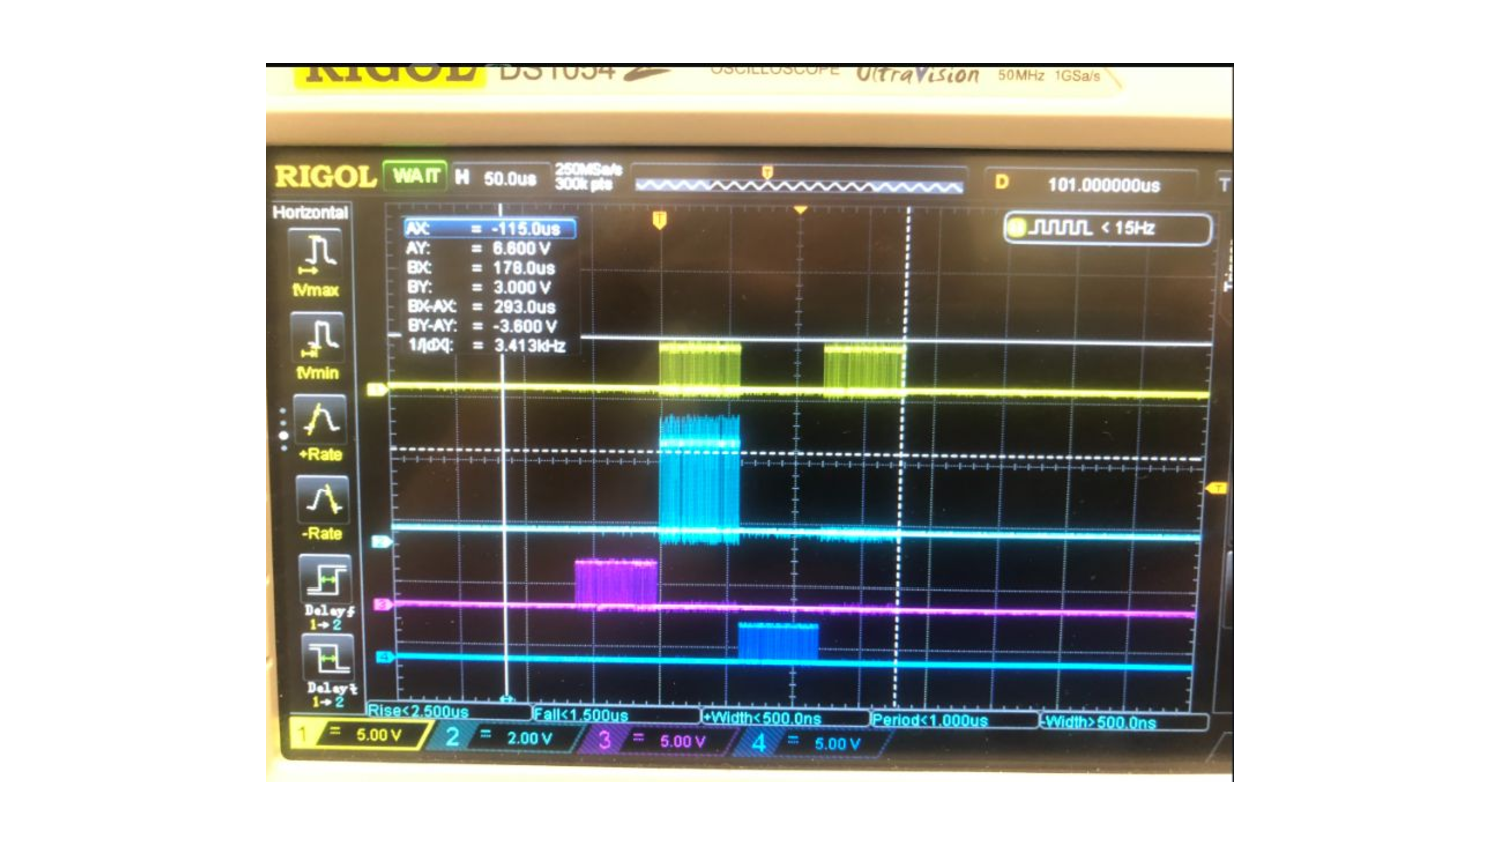
\includegraphics[width=\textwidth]{images/qdb_example_packet_waveform.pdf}
  \caption{Waveforms caught on an oscilloscope. The timescale is 50 $\unit{\mu s}$.}
\end{subfigure}%
\begin{subfigure}{.5\textwidth}
  \centering
  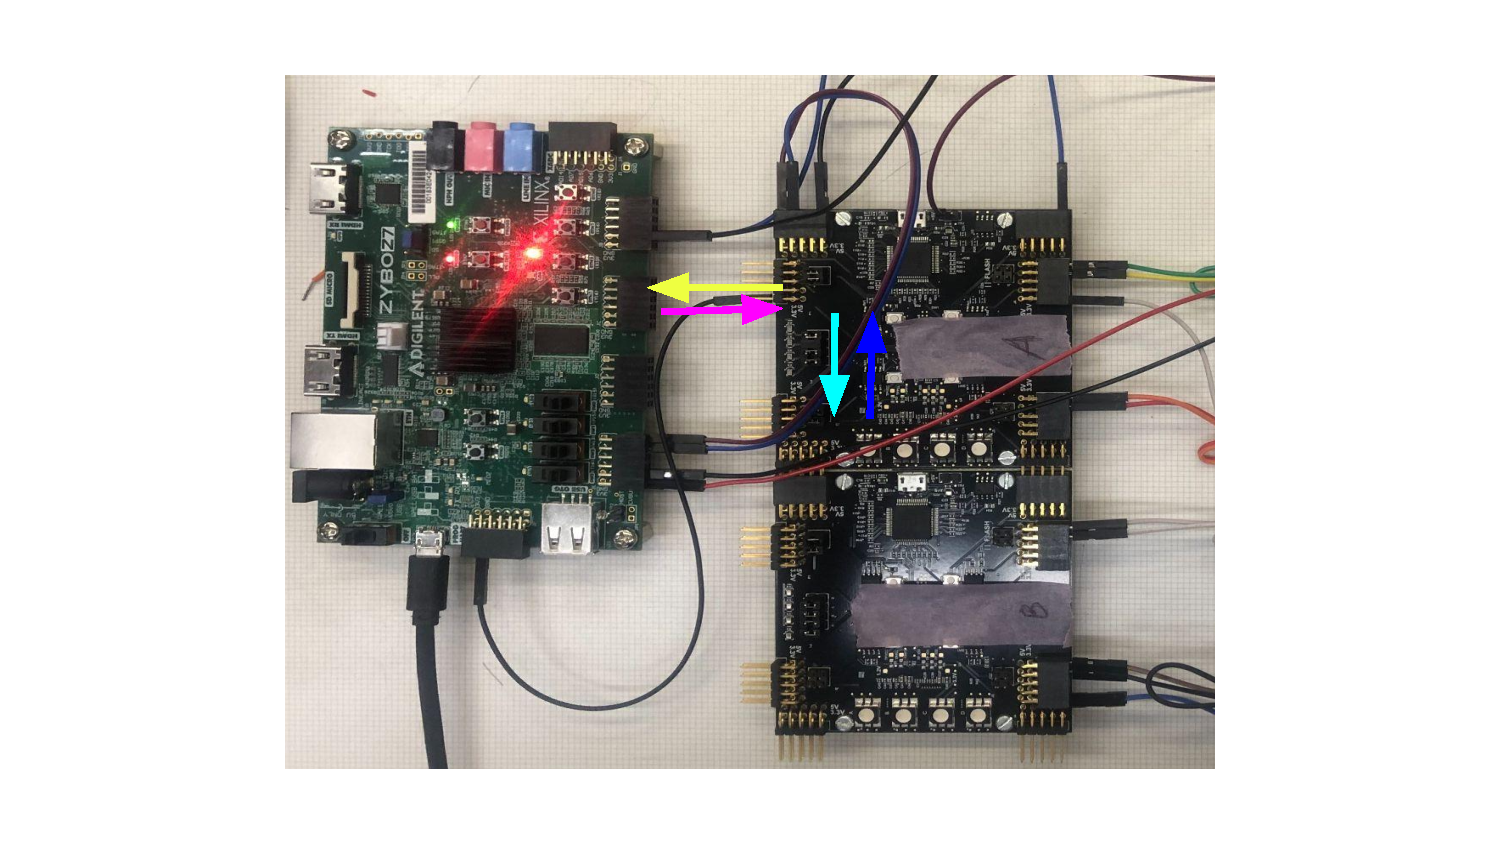
\includegraphics[width=\textwidth]{images/qdb_example_packet_waveform_diagram.pdf}
  \caption{Communication Route on Prototype}
\end{subfigure}
\caption{}
\end{figure}



\subsection{Frequency Calibration of each Node}


%% 4Hz interrogation calibration 
\begin{table}
	\begin{center}
		\begin{tabular}{|c|c|c|c|}
			\hline
			FPGA Position & Mean (30~\unit{MHz}) & STD & $\frac{\delta f}{f_{o}}$*1e6 (ppm) \\
			\hline
			(0,0) & 245.543 & 2.379 & 0.079 \\
			\hline
			(0,1) & 190.646 & 2.979 & 0.099 \\
			\hline
			(0,2) & 153.908 & 3.334 & 0.111 \\
			\hline
			(0,3) & 248.831 & 3.843 & 0.128 \\
			\hline
			(1,0) & 192.729 & 2.860 & 0.095 \\
			\hline
			(1,1) & 210.905 & 3.405 & 0.114 \\
			\hline
			(1,2) & 116.212 & 3.984 & 0.133 \\
			\hline
			(1,3) & 159.824 & 4.158 & 0.139 \\
			\hline
			(2,0) & 351.431 & 3.685 & 0.123 \\
			\hline
			(2,1) & 193.845 & 4.285 & 0.143 \\
			\hline
			(2,2) & 200.278 & 4.071 & 0.136 \\
			\hline
			(2,3) & 152.633 & 4.263 & 0.142 \\
			\hline
			(3,0) & 183.359 & 3.954 & 0.132 \\
			\hline
			(3,1) & 209.788 & 4.561 & 0.152 \\
			\hline
			(3,2) & 192.277 & 4.169 & 0.139 \\
			\hline
			(3,3) & 171.302 & 4.538 & 0.151 \\
			\hline
		\end{tabular}
	\end{center}
	\caption{FPGA calibration results based on Hard Intterrogations at a frequnecy of 4~\unit{Hz}.
	The mean and standard deviation (STD) values are reconstructed for each ASIC within the tile as done in Figure~\ref{fig:frq_recon_node00} and ~\ref{fig:frq_recon_node33}.
	The listed STD value is the result of a gaussian fit performed on the adjusted frequencies.
	}
	\label{tab:fpga_calibration}
\end{table}

\begin{figure}[]
\centering
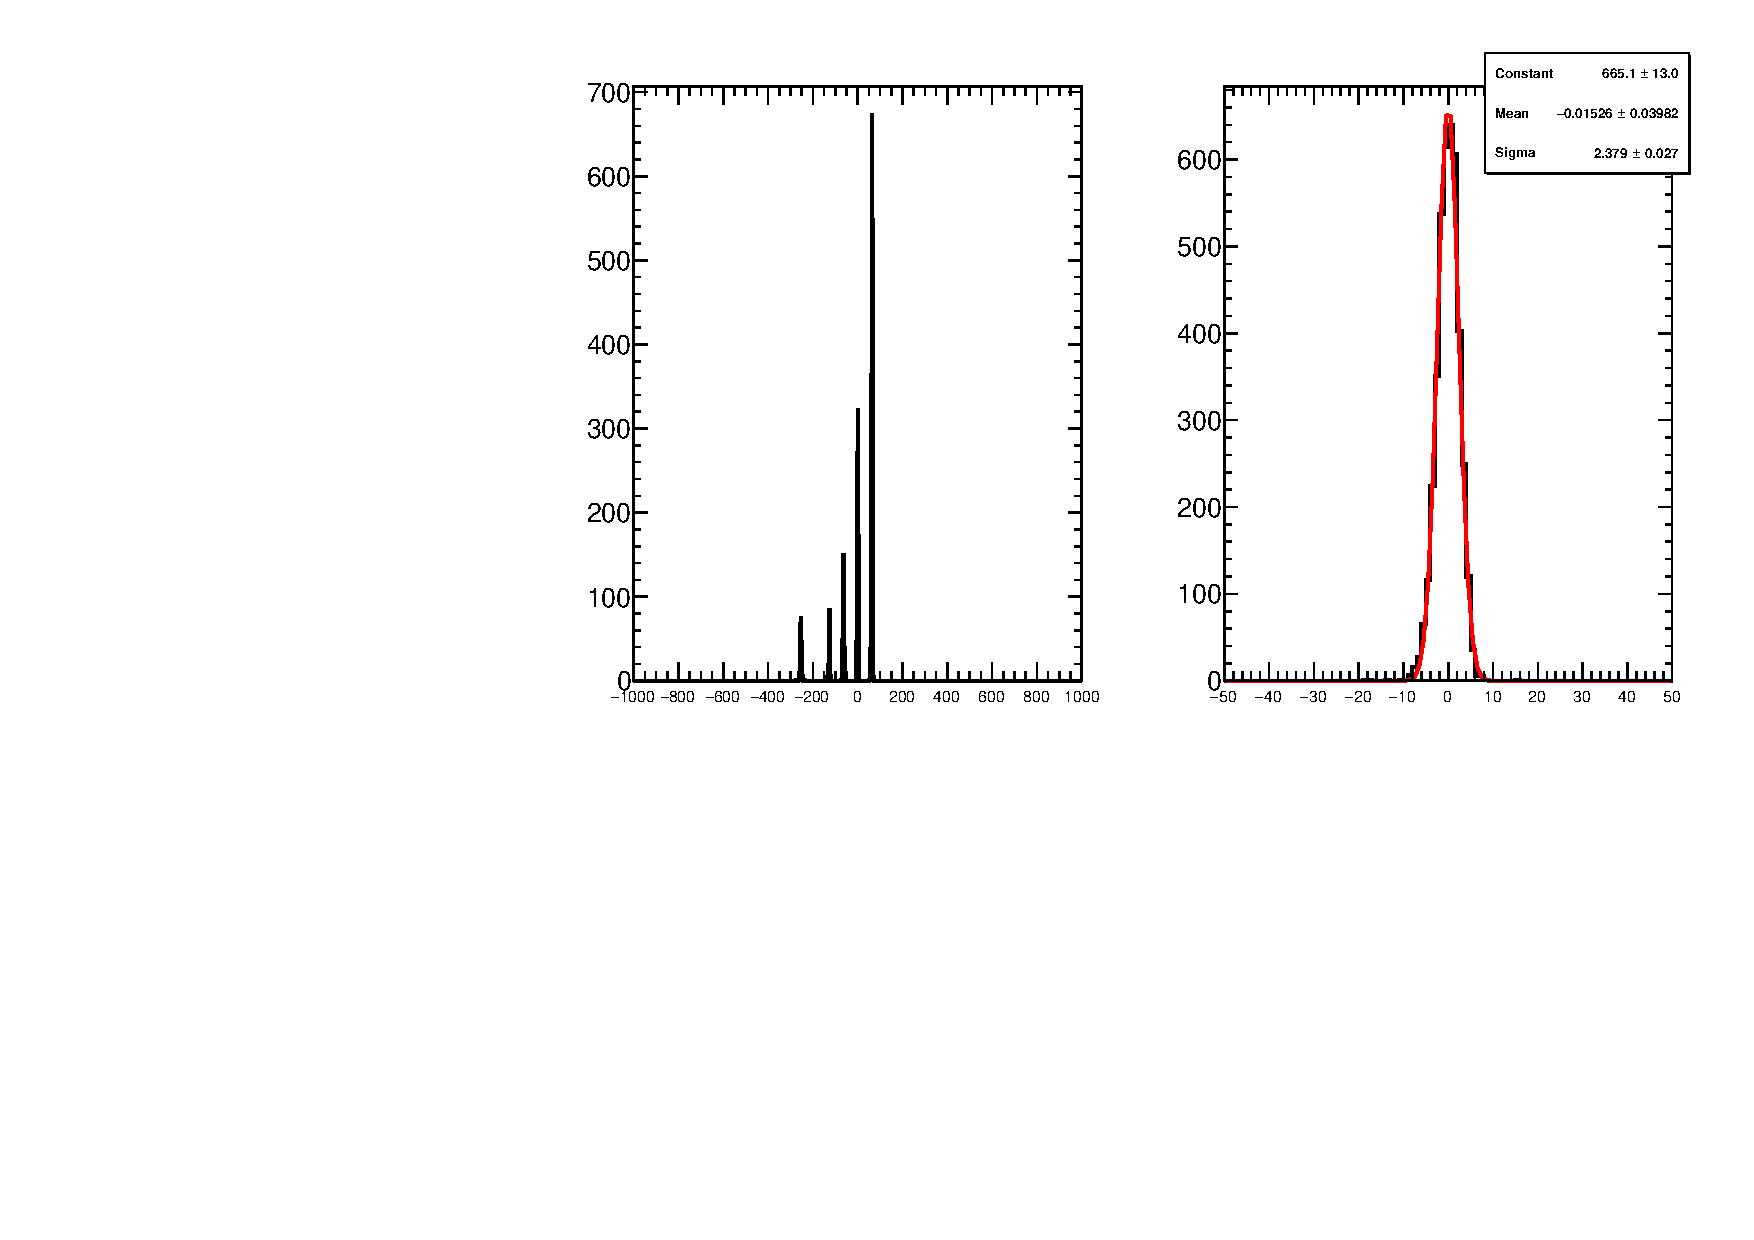
\includegraphics[width=0.9\textwidth]{images/(0,0).pdf}
\caption{Example of frequency calibrations for the FPGA Adjacent to the Zybo.}
\end{figure}

\begin{figure}[]
\centering
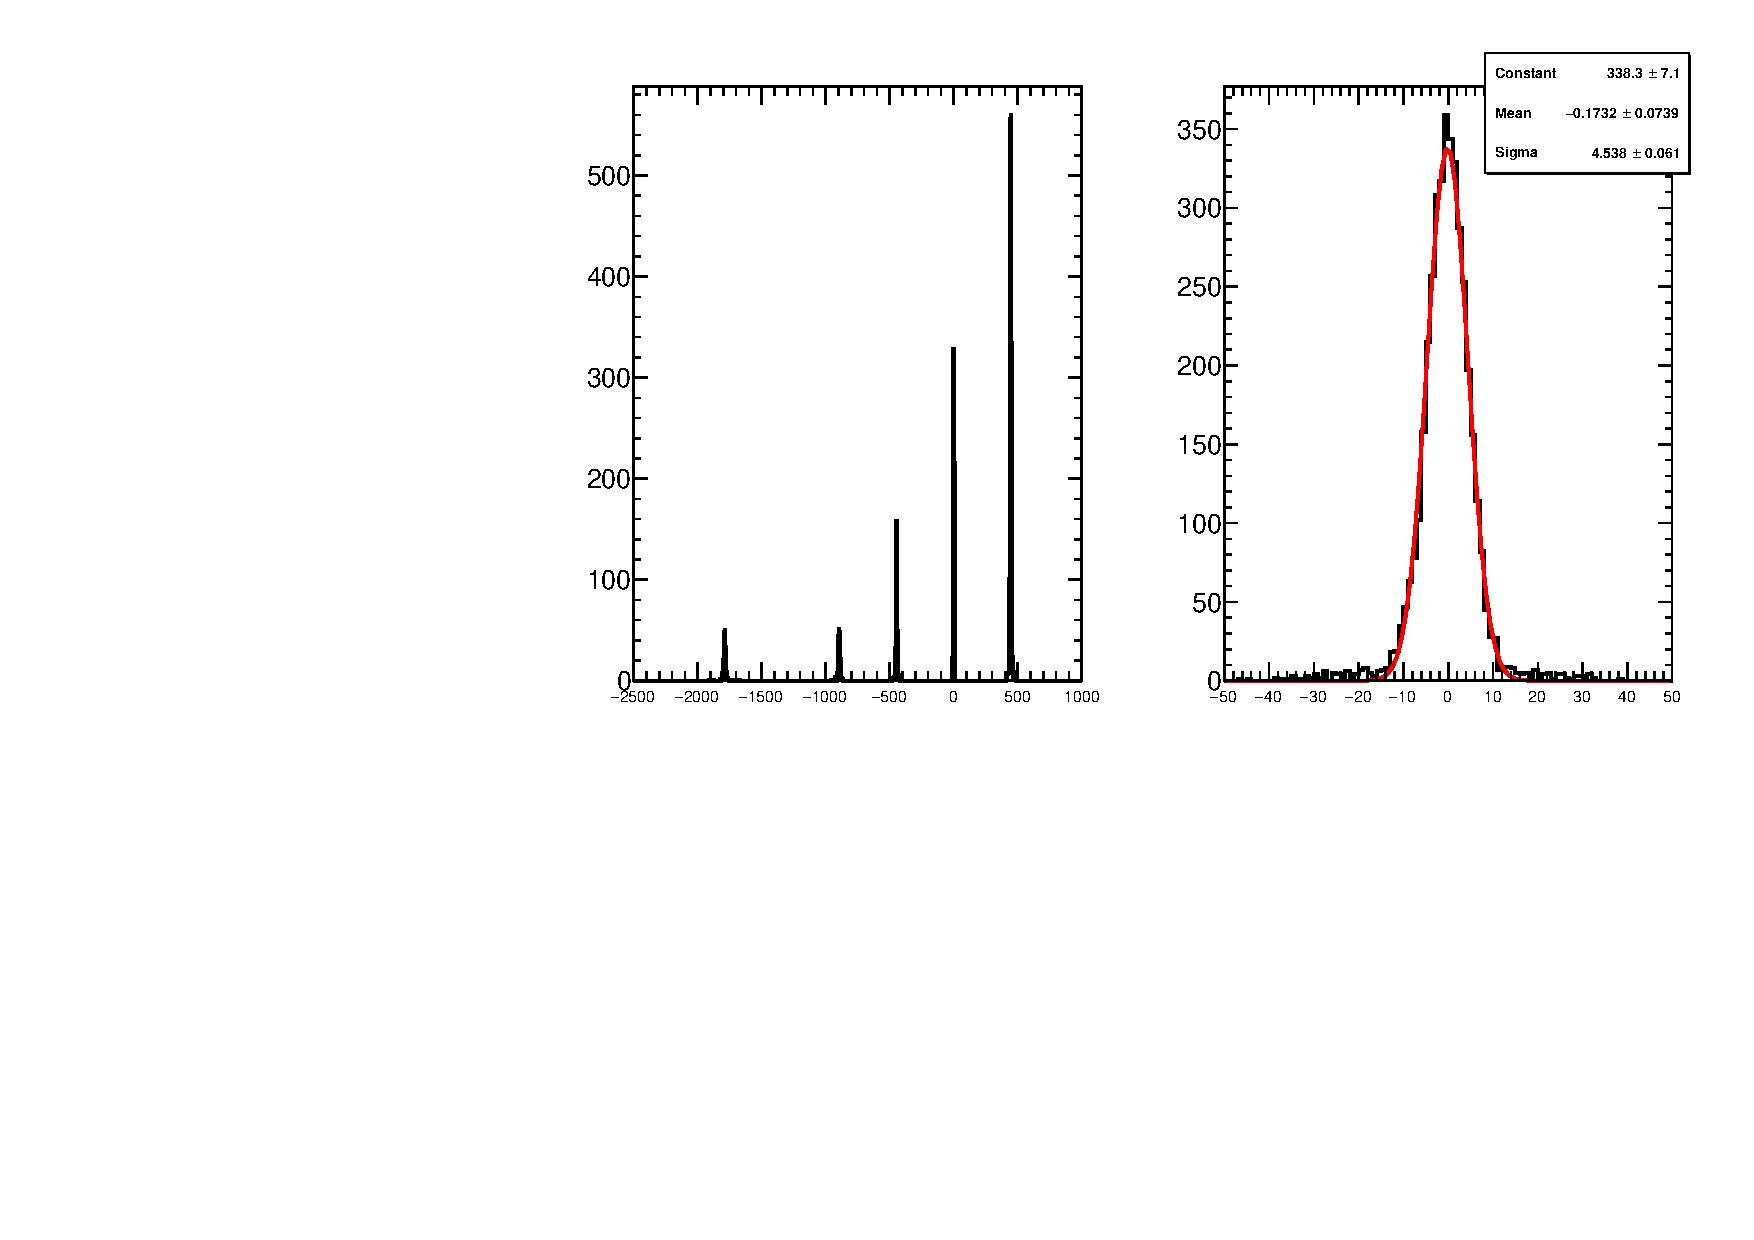
\includegraphics[width=0.9\textwidth]{images/(3,3).pdf}
\caption{}
\end{figure}

\begin{figure}[]
\centering
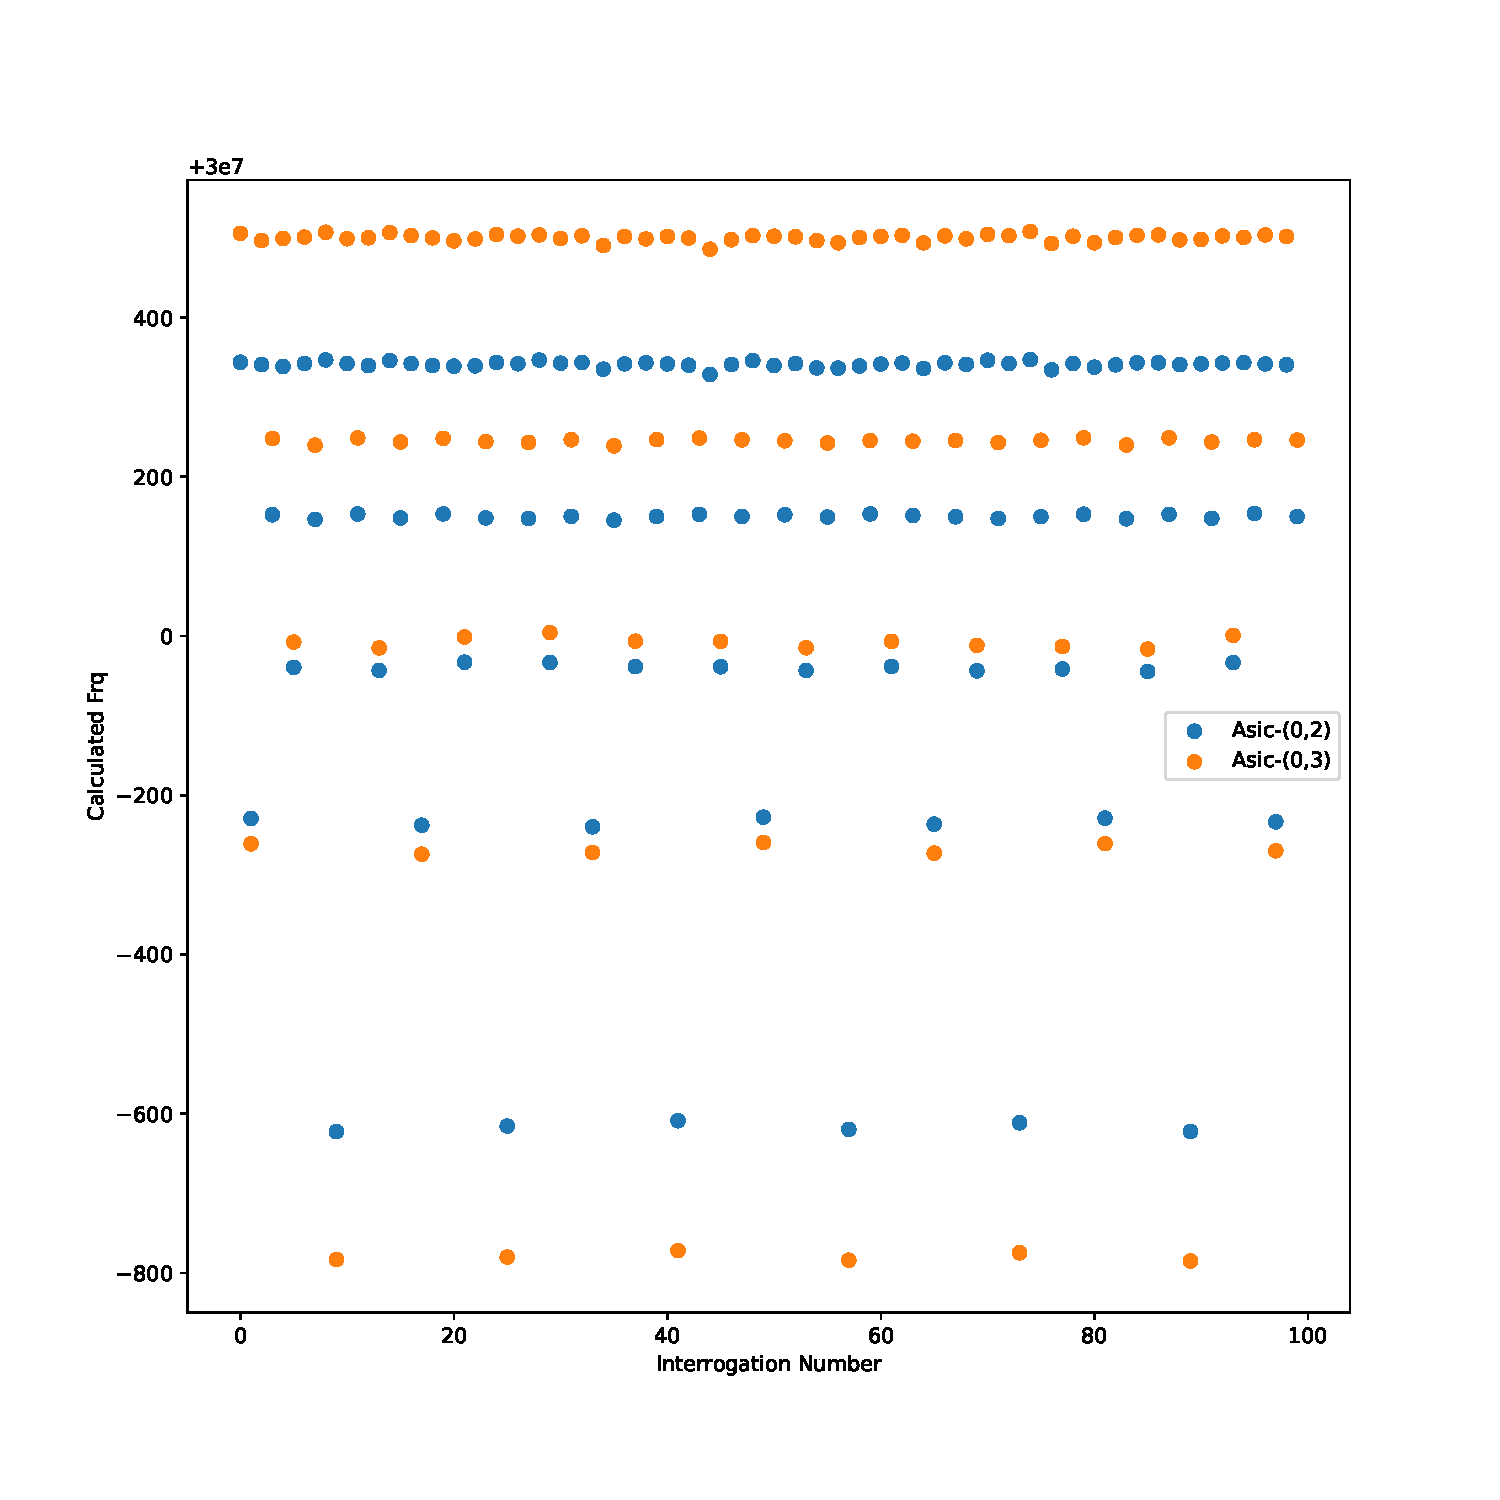
\includegraphics[width=0.9\textwidth]{images/fast_example.pdf}
\caption{}
\end{figure}

\begin{figure}[]
\centering
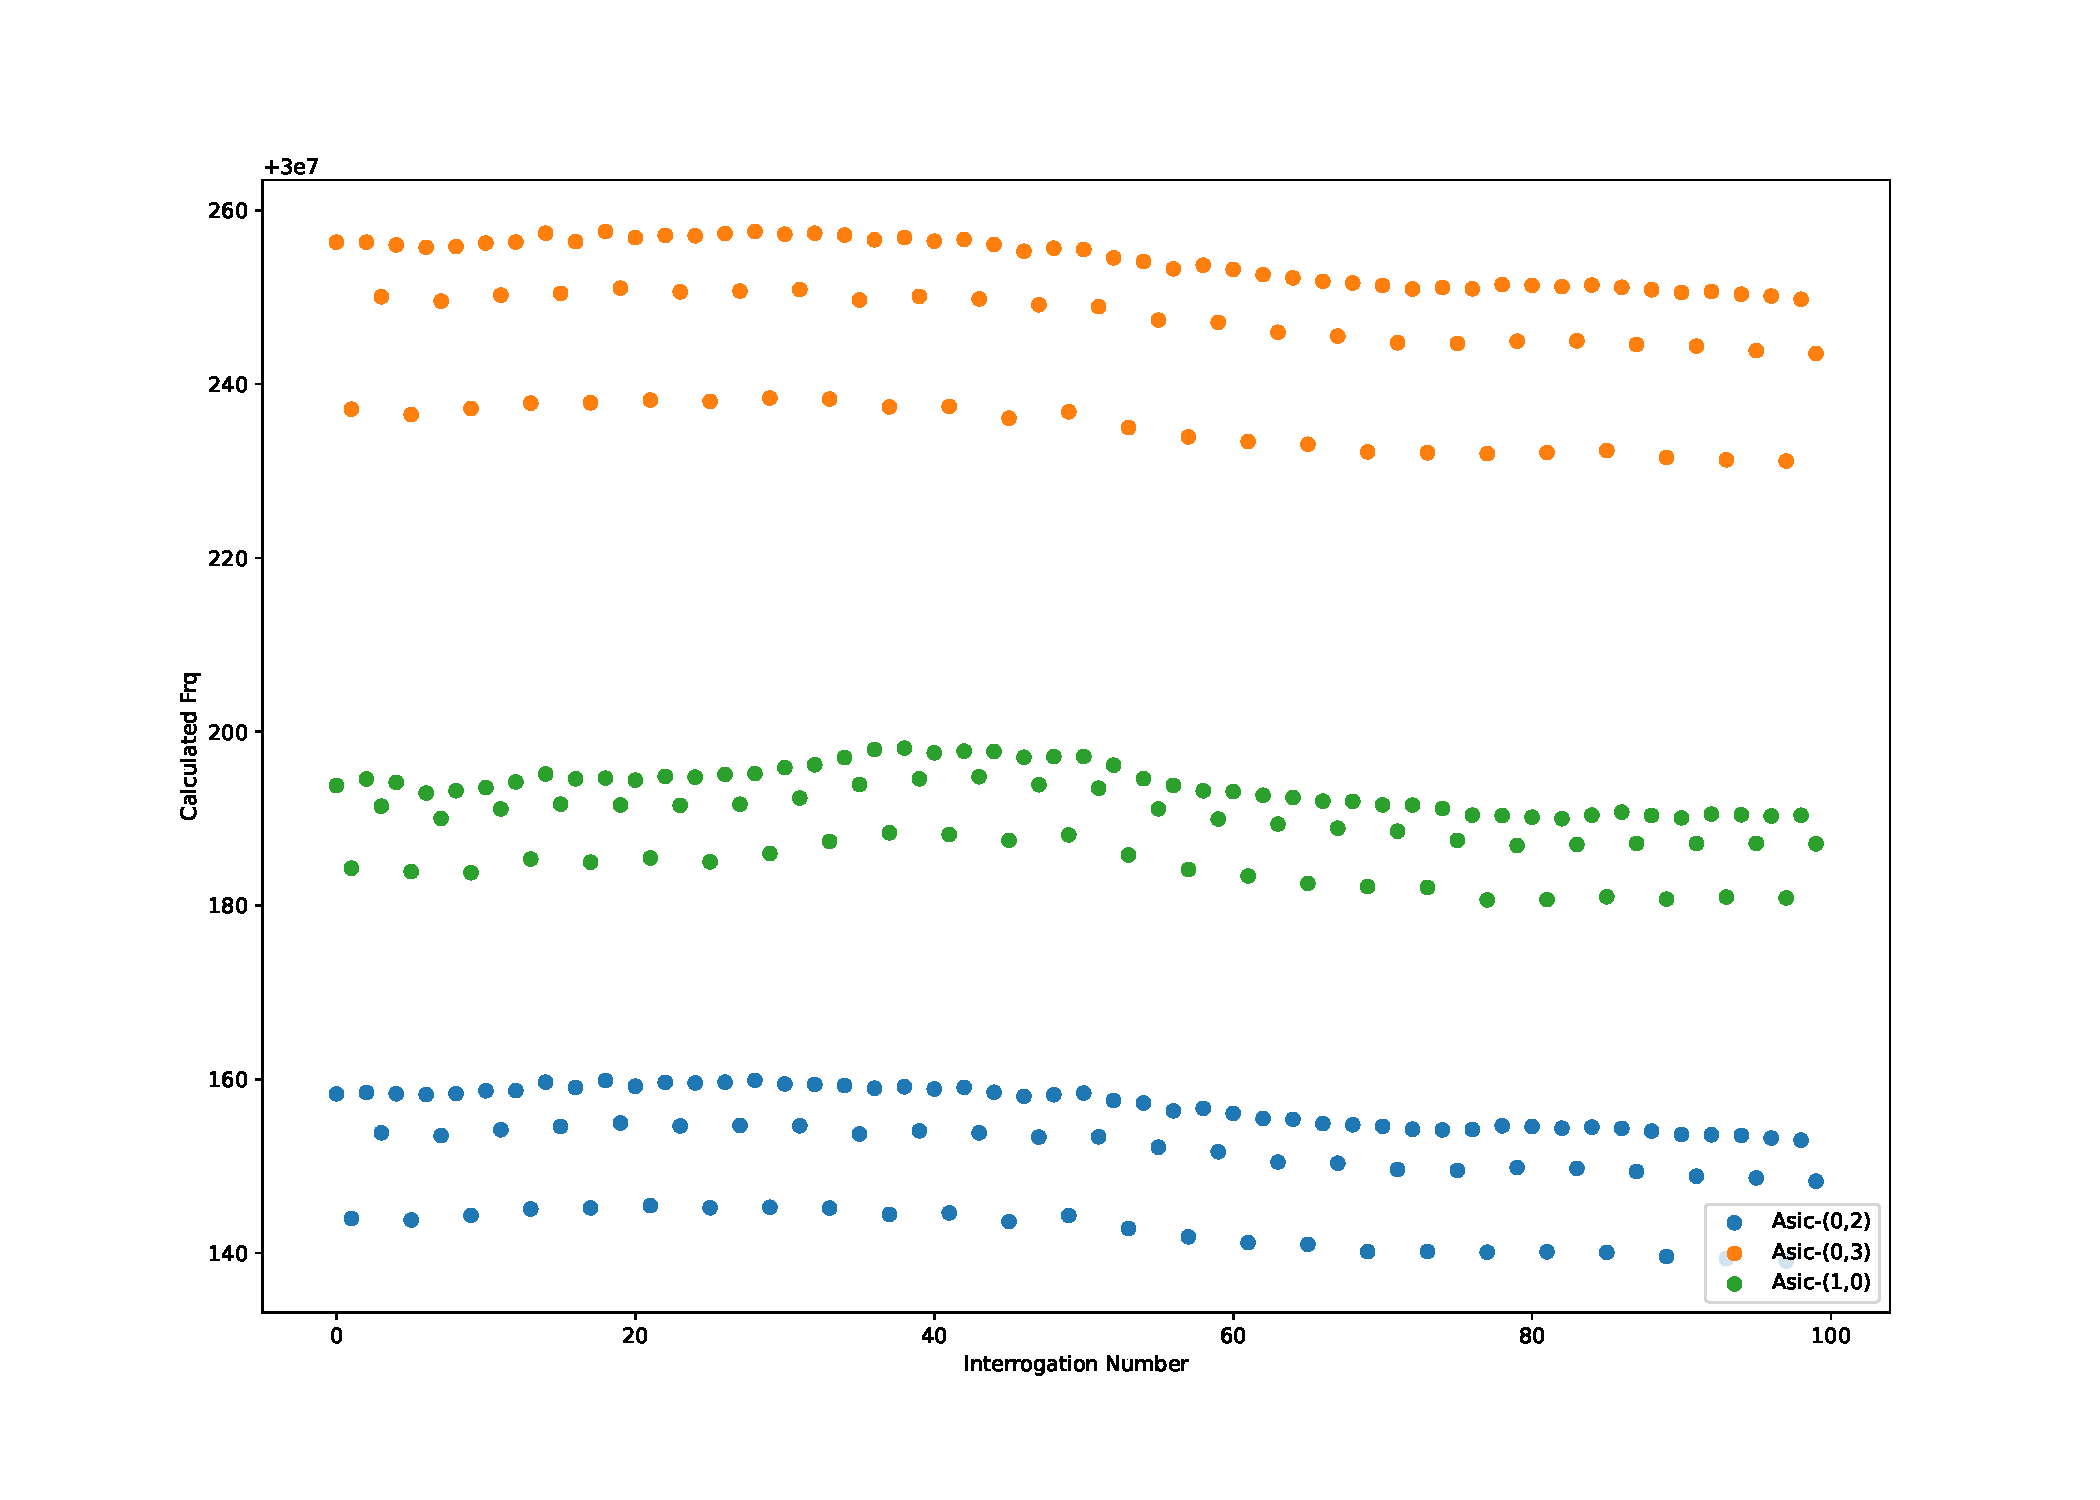
\includegraphics[width=0.9\textwidth]{images/slow_example.pdf}
\caption{}
\end{figure}


%% 0.1 Hz interrogation calibration 
\begin{table}
	\begin{center}
		\begin{tabular}{|c|c|c|c|}
			\hline
			FPGA Position & Mean (30~\unit{MHz}) & STD & $\frac{\delta f}{f_{o}}$*1e6 (ppm) \\
			\hline
			(0,0) & 243.223 & 3.895 & 0.130 \\
			\hline
			(0,1) & 187.225 & 4.631 & 0.154 \\
			\hline
			(0,2) & 151.020 & 6.255 & 0.208 \\
			\hline
			(0,3) & 246.553 & 8.229 & 0.274 \\
			\hline
			(1,0) & 188.851 & 4.521 & 0.151 \\
			\hline
			(1,1) & 207.837 & 6.468 & 0.216 \\
			\hline
			(1,2) & 111.344 & 7.882 & 0.263 \\
			\hline
			(1,3) & 156.660 & 9.985 & 0.333 \\
			\hline
			(2,0) & 348.263 & 6.748 & 0.225 \\
			\hline
			(2,1) & 190.976 & 8.622 & 0.287 \\
			\hline
			(2,2) & 196.369 & 9.919 & 0.331 \\
			\hline
			(2,3) & 148.284 & 11.844 & 0.395 \\
			\hline
			(3,0) & 179.718 & 8.375 & 0.279 \\
			\hline
			(3,1) & 207.859 & 10.655 & 0.355 \\
			\hline
			(3,2) & 188.123 & 11.836 & 0.395 \\
			\hline
			(3,3) & 165.011 & 13.725 & 0.457 \\
			\hline
		\end{tabular}
	\end{center}
	\caption{FPGA calibration results based on hard interrogations at a frequnecy of 0.1~\unit{Hz}.
	These data are more tightly clusted together due to the longer wait time between each interrogation, and are not easily separable as done in Table~\ref{tab:fpga_calibration}.
	The listed mean is the simple geometric mean and standard deviation for a one hour run time.
	}
	\label{tab:fpga_slow_calibration}
\end{table}


%% schematic of PCB

\section{Timing Stability and Communication Verification}~\label{sec:timing_test_results}

We describe here the methods of measuring a stable time for different configurations of the nodes.
We also comment on the results of the timing with resepect to the minimum required timing sensitivity in order to have accurate timestamp reconstruction.

\begin{figure}[]
\centering
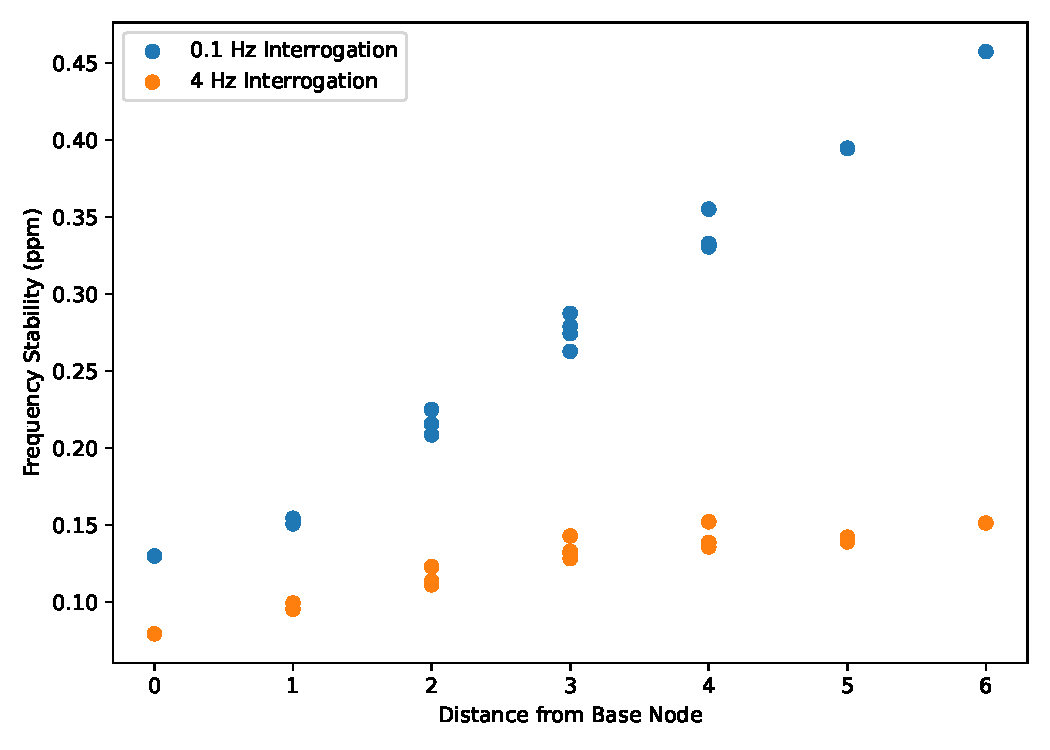
\includegraphics[width=0.9\textwidth]{images/interrogation_ppm_diff.pdf}
\caption{}
\end{figure}

\section{Power and Current Characteristics}

There are test pads on the PCBs used to measure the voltage stability of the different FPGA voltages.
For each voltage, there is also a single 1~$\unit{\Omega}$ probe-resistor.
This resistor is used to measure the relative current drawn from each of the voltage sections on the PCB.

\section{Analysis of Systematics for Different System Implementations}

The essential features of the digital node in the Q-Pix readout are the properties of the local oscillator.
The frequency, relative phases, and stability of the oscillator determine the power consumption, packet transaction time, minimum timestamp resolution, which determines maximum current measurements, and affects packet loss probability in larger tile systems.
It is not an understatement to say that the successful development of the digital node relies on the development of the local oscillator.

\section{Towards the Integration of the Aggregator Node}

In the studies presented here, The aggregator node which was used was the Zybo Z7-20.

\section{Comments on A Super-DAQ-Node}

Each APA module within a larger DUNE module must ultimately be interconnected so that the entire module can be readout.
As described above, a single modular tile is controlled by an individual DAQ node, where many constitute a complete APA.
Therefore, we refer to the device that digitally multiplexes all of the DAQ node data as the "Super DAQ Node" (SDN).
Then, we imagine the final multiplexing stage for an entire DUNE module as an array of SDNs, each of which consistute an array of DAQ nodes, where each DAQ node is a 2-D array of Q-Pix based ASICs.

The total number of request SDNs within the full dune module depends on the final size of a DAQ-node controlled tile.

%% high level figure here from TPC -> Integrator -> Digital Node -> Aggregator -> SuperDAQ-Node -> WIC -> Disc

\section{The Back-End Summary}
